\section{Einleitung}


Lorem\marg{Ausgangssituation} Lorem dolor sit amet, consetetur sadipscing elitr, sed diam nonumy eirmod tempor invidunt ut labore et dolore magna aliquyam erat, sed diam voluptua. At vero eos et accusam et justo duo dolores et \autocite[22]{Roppel2006} ea rebum. Stet clita kasd gubergren, no sea \textbf{\ref{tab:Hochwasserszenarien}} takimata sanctus est Lorem ipsum dolor sit amet. Lorem ipsum dolor sit amet, consetetur sadipscing elitr, sed diam nonumy eirmod tempor invidunt ut labore et dolore magna aliquyam erat, sed diam voluptua. At vero eos et accusam et justo duo dolores et ea rebum. Stet clita kasd gubergren, \textbf{\ref{fig:HSR}} no sea takimata sanctus est Lorem ipsum dolor sit\footcite{Roppel2006} \textbf{\ref{eq:Hochwasserzufluss}} amet.\footfullcite{Roppel2006}

\begin{figure}[ht]
	\centering
	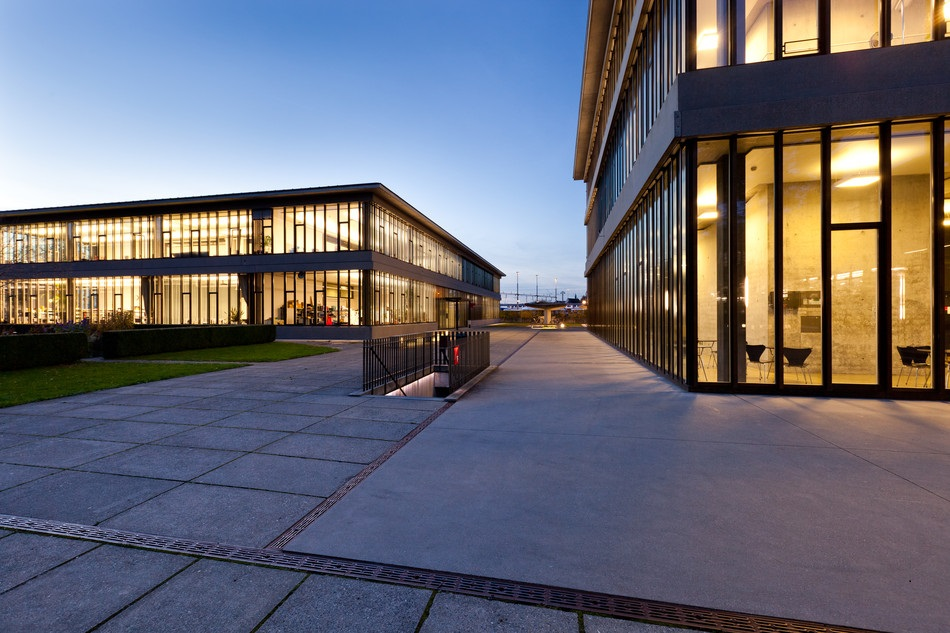
\includegraphics[width=0.6\textwidth]{images/hsr.jpg}
	\caption{\acs{HSR} \autocite{IR}}
	\label{fig:HSR}
\end{figure}

Lorem\marg{Was ist das Problem?}

 \begin{equation}\label{eq:Hochwasserzufluss}
\frac{Q(t)}{Q_{max}} = \left(\frac{t}{t_max}\cdot e^{1-\frac{t}{t_max}} \right)^n
\end{equation}
\myequations{Definition Hochwasserzufluss}

\begin{table}[ht]
    \centering
	\begin{tabular}{|l|l|l|l|l|l|}
		\hline 
		\textbf{Ganglinie}	&\textbf{[ ... ]}  	& \textbf{A} 	 & \textbf{B}  	& \textbf{C} 	& \textbf{D}  \\ 
		\hline 
		$ Q_{max} $			& $ m^3/s $ 		& 50 			& 70		  	& 180			& 540 \\ 
		\hline 
		$ t_{max} $			& $ h $ 			& 2  			& 2 			& 3 			& 4 \\ 
		\hline 
		n					& --  				& 6  			& 6 			& 6 			& 6  \\ 
		\hline 
	\end{tabular} 
	\caption{Hochwasserszenarien}\label{tab:Hochwasserszenarien}
\end{table}

Lorem \marg{Ziel} Lorem dolor sit amet, consetetur sadipscing elitr, sed diam nonumy ei\\

Lorem \marg{Wie soll das Problem gelöst werden?} Lorem dolor sit amet, consetetur sadipscing elitr, sed diam nonumy ei \\
\ac{HSR}\\
\acs{HSR}\\
\acl{HSR}


\clearpage